% 93-23(93쪽) — 변 BC 위에 점 D 가 있는 삼각형 ABC(원문 「오른쪽 그림」). 스캔 화질이 낮아 TikZ 로 다시 그림.
% 라벨은 원문 것만: 꼭짓점 A·B·C·D, 길이 4·6·5·3. 선분 AD 의 길이(답)는 그림에 적지 않는다.
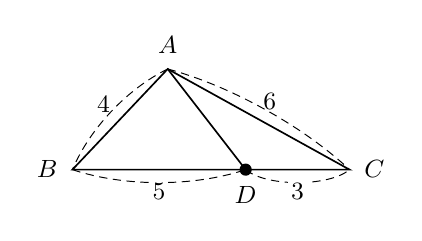
\begin{tikzpicture}[line width=0.6pt, x=0.44cm, y=0.44cm]
  \coordinate (A) at (2.75,2.905);
  \coordinate (B) at (0,0);
  \coordinate (C) at (8,0);
  \coordinate (D) at (5,0);
  \draw (A) -- (B) -- (C) -- cycle;
  \draw (A) -- (D);
  \fill (D) circle (2.2pt);
  % 길이 표시의 점선 호
  \draw[densely dashed, line width=0.35pt] (A) .. controls (1.595,2.344) and (0.495,1.182) .. (B);
  \draw[densely dashed, line width=0.35pt] (A) .. controls (4.543,2.428) and (6.643,1.266) .. (C);
  \draw[densely dashed, line width=0.35pt] (B) .. controls (1.50,-0.50) and (3.50,-0.50) .. (D);
  \draw[densely dashed, line width=0.35pt] (D) .. controls (5.60,-0.50) and (7.40,-0.50) .. (C);
  \node[font=\small, anchor=south] at (2.75,3.05) {$\pt{A}$};
  \node[font=\small, anchor=east] at (-0.14,0.02) {$\pt{B}$};
  \node[font=\small, anchor=west] at (8.14,0.02) {$\pt{C}$};
  \node[font=\small, anchor=north] at (5.00,-0.20) {$\pt{D}$};
  \node[font=\small] at (0.90,1.88) {$4$};
  \node[font=\small] at (5.70,1.98) {$6$};
  \node[font=\small, fill=white, inner sep=1pt] at (2.50,-0.62) {$5$};
  \node[font=\small, fill=white, inner sep=1pt] at (6.50,-0.62) {$3$};
\end{tikzpicture}
